%-------------------------------------------------------------------------------
\section{Introduction}
\label{s:intro}
%-------------------------------------------------------------------------------

Providers like best effort (BE) workloads, because these allow them to get high
utilization by oversubscribing their machines without compromising any
guarantees: Under high load, latency critical (LC) workloads run without
impediment, but in low load BE runs opportunistically and the servers maintain
high utilization.\hmng{it's not just providers though, b/c what about people
running their own kubernetes deployment... but it's also not really developers}
This is why for example, in recent measures, around XX\% of the workload running
in YY was BE.

Dynamically reallocating CPUs as the load changes is challenging: the scheduler
needs to maintain low latencies for LC requests by ensuring that when the LC
processes need resources they appear uncontended, while at the same time using
idle resources to run BE processes.

The current standard mechanism for isolating LC from BE processes is Linux's
\cgroups{}. This includes all Open Container Initiative (OCI) compliant
containers, such as Docker, Kubernetes, CRI-O, and containerd, because the OCI
specification calls for use of \cgroups{}. VMs, including Firecracker, AFaas,
and KVM, also rely on \cgroups{} to manage VMs when the number of vCPUs is
oversubscribed.

The interface \cgroups{} exposes in order to specify the priority of processes
is based on weight: each workload is put into its own group, and each group is
assigned a weight in the range [1, 10000]. Under the hood, Linux runs a weighted
fair share scheduling algorithm. Other operating systems use a similar
interface, for instance Windows exposes a number of shares. 

\begin{figure}[t]
    \centering
    \begin{subfigure}[b]{0.49\columnwidth}
        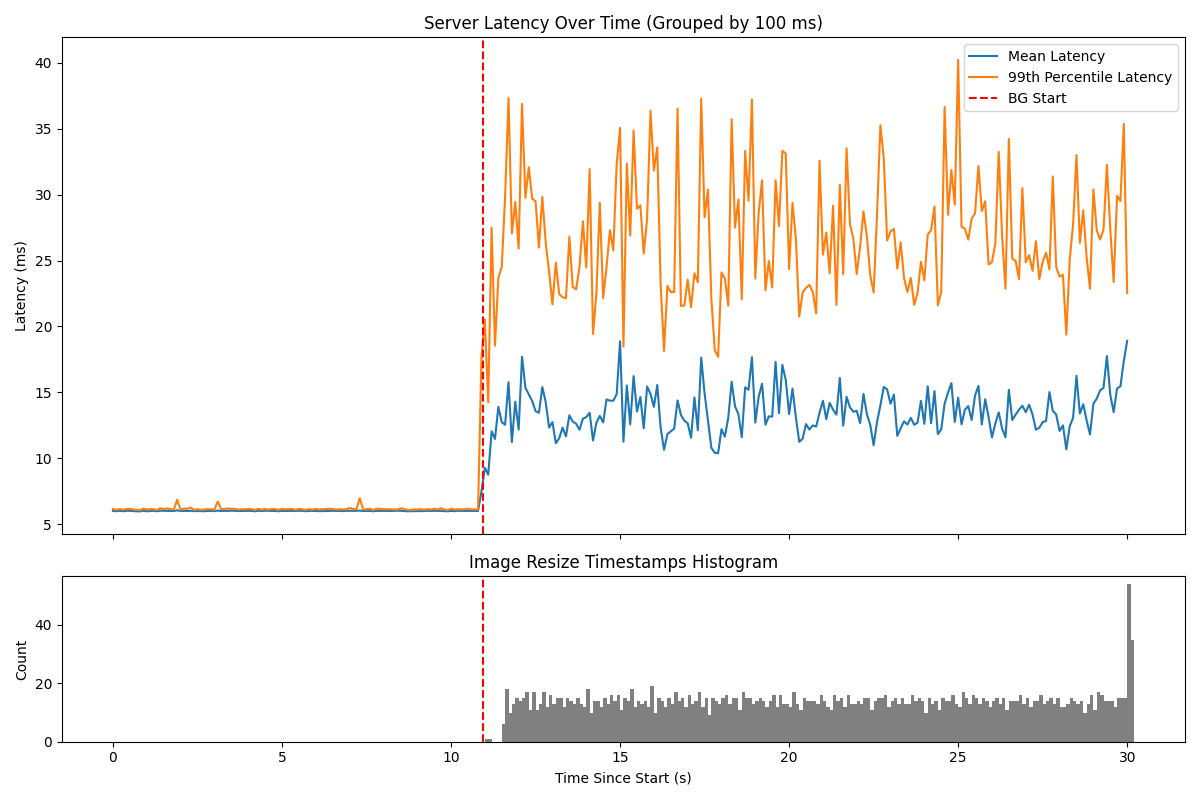
\includegraphics[width=\columnwidth]{graphs/unedited-weight-low-two.png}
        \caption{Low load stetting, utilization before starting the BE tasks is
        around 85\%}\label{fig:unedited-weight-low-two}
    \end{subfigure}
    \hspace{\fill}
    \begin{subfigure}[b]{0.49\columnwidth}
        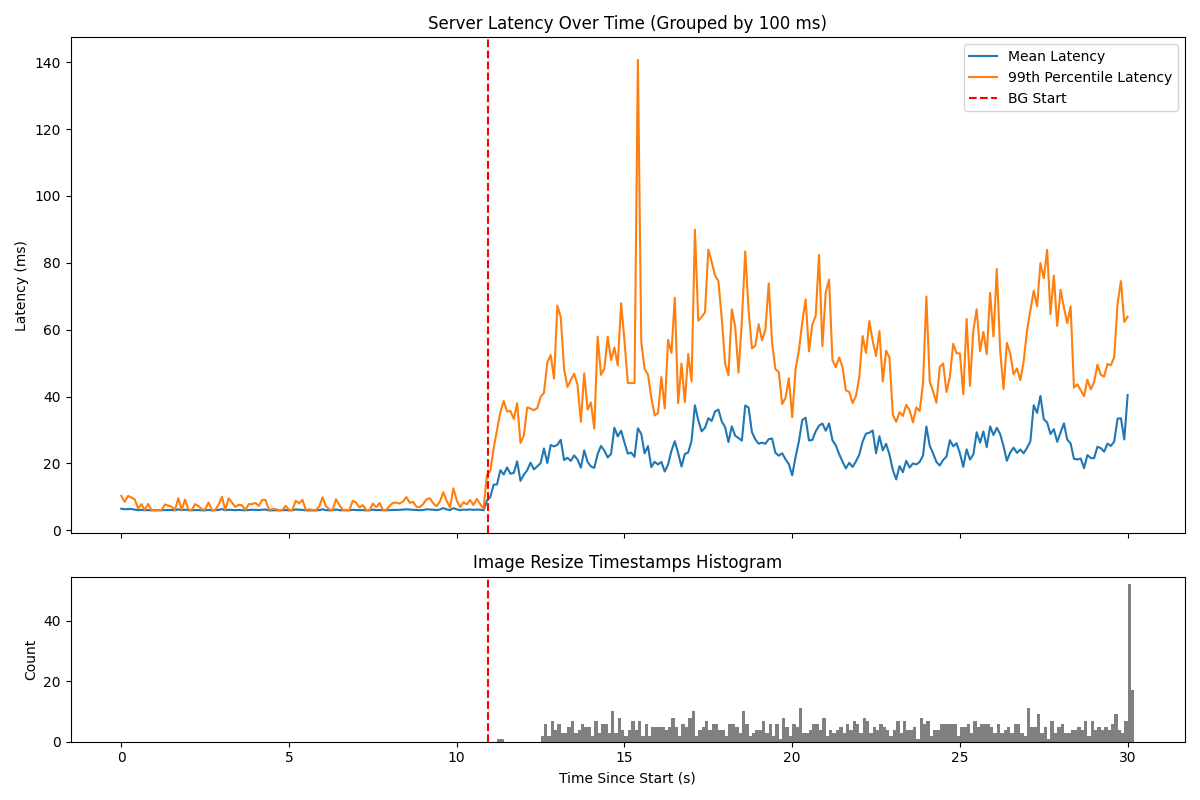
\includegraphics[width=\columnwidth]{graphs/unedited-weight-high-two.png}
        \caption{High load setting, utilization before starting the BE tasks is
        around 95\%}\label{fig:unedited-weight-high-two}
    \end{subfigure}
    \vspace{4pt}
    \caption{Latencies of the server and iteration counts of the background
    tasks in different load scenarios. Note the different y axis limits. The
    upper graphs show end-to-end request latencies, and the bottom graph is a
    histogram of completed iterations of the BE tasks}\label{fig:unedited-weight}
\end{figure}

In principle, this range is large, and should allow for BE tasks to have a
negligible performance impact on LC tasks, even during high load. However, we
find that the presence of low weight (ie BE) tasks has a large performance
impact on a high-weight (ie LC) task. In an experiment, we run a simple
cpu-bound server and then start two BE workloads doing image resizing.
\autoref{fig:unedited-weight} shows the increase in latencies of the LC server
at two different baseline utilization levels. We see that mean latencies spike
up from steady at just under 6ms to as high as 13ms, and much higher for 99th
percentile latencies. We explore the reasons for this behavior in detail in
\autoref{s:problem}, with the main takeaway being that Linux fails to enforce
weights across cores.

In this paper, we argue that the split between LC and BE should be categorical
rather than ends of a weight spectrum, and that unfairness should be the goal.
We implement the desired policy in Linux by modifying an existing mostly unused
scheduling policy called \schedidle{}, and show that doing so enables Linux to
isolate LC from BE: in the same experiment, the increase in average latency when
starting a BE workload goes from $\sim x 2$ to none, and the tail latency XX.
The contributions of this paper are thus as follows: 
\begin{enumerate}
    \item the insight that weighted fair share breaks down with large weight
    splits because the weights are not enforced across cores; and that this
    dramatically affects end-to-end latencies
    \item showing that enforcing weights across core is prohibitively expensive,
    but categorical priorities are simpler to enforce, and that Linux does this
    well
    \item a patch to Linux that effectively creates a fully separated scheduling
    class that BE tasks can run in, which isolates LC workloads get from BE ones
    and minimizes the amount of added latency to do cross-core checks
\end{enumerate}
